%Computing counts, N1+ of several flavours of different sized n-grams.

The key requirements for computing probability under a Kneser-Ney language model are two types of counts: raw frequencies of \ngrams and occurrence counts, quantifying in how many different contexts the \ngram has occurred.%
\footnote{The need such counts is not specific to Kneser Ney, indeed
  many other smoothing variants for \ngram LMs impose similar
  requirements and could be computed straightforwardly using the algorithms below.}
Figure~\ref{fig-counts-example} (right) illustrates the numbers needed in calculating the probability of an example 4-gram.
By electing to store the corpus directly in a suffix tree, we need to provide mechanisms for computing these counts based on queryies into the suffix tree.

The raw frequency counts are the simplest to compute. First we
identify the node in the suffix tree labelled with the query
\ngram; the frequency corresponds to the node's \emph{size}, defined as the
distance between its left and right bounds (corresponding to the
number of descendents under the node). To illustrate, consider
searching for \emph{the night} in  Figure~\ref{fig-suffix-tree}, which
matches a node with two descendents (labelled 19 and 12), and thus the
\ngram has count 2. This is a simple $\Order{1}$ operation once the
node has been identified.

More problematic are the occurrence counts, which come in several
flavours: with the dot to the right of the pattern, $\nlplus{\patdot}$,
to the left,  $\nlplus{\dotpat}$, and on both sides
$\nlplus{\dotpatdot}$. The first of these can be handled easily, by
querying the \emph{degree} of the matching node in the suffix tree. E.g., 
\emph{keep in} has two child nodes in  Figure~\ref{fig-suffix-tree},  
and thus there are two unique contexts in
which it can occur, $\nlplus{\emph{keep in~}\Bigcdot}=2$. This follows naturally from the suffix tree
construction, where all descendent nodes correspond to larger \ngrams with
same prefix, and each child edge extends the \ngram with a different
subsequent symbol. 
%
\begin{algorithm}[t]
  \caption{Compute one-sided occurrence counts, $\nlplus{\dotpat}$ or $\nlplus{\patdot}$ for pattern $\alpha$ 
    \label{alg:n1plus}}
  \begin{algorithmic}[1]
    \Require{node $n$ in \CST $t$ matches $\alpha$}
    \Function{N1Plus}{$t, n, \alpha$} %\Comment{ $t$ is either forward or reverse \CST}
        \Let{$o$}{$0$} %\Comment{yielding $\nlplus{\patdot}$ or $\nlplus{\dotpat}$, respectively}
        %\If{$\leaf{t}{n} \, \wedge \, \depth{t}{n} = |\alpha|$}
        \If{$\depth{t}{n} = |\alpha|$}
          \Let{$o$}{$\degree{t}{n}$}
        \Else
          \Let{$o$}{$1$}
        \EndIf
      \State \Return{$o$}
    \EndFunction
  \end{algorithmic}
\label{alg-nlplus}
\end{algorithm}
%
A similar line of reasoning applies to computing
$\nlplus{\dotpat}$. Assuming we also have a suffix tree representing
the \emph{reversed corpus}, we can easily identify the reversed pattern
(e.g., \emph{in keep}) and query the degree for the matching node. This
approach is illustrated in Algorithm~\ref{alg-nlplus}, where we first
test if the node matches the pattern completely, i.e., its
\emph{depth} corresponds to the pattern length, in which case we use
the degree;\footnote{There are some corner cases involving sentinels \#
  and \$, which aren't counted in computing unique contexts.
  Such tests have been omitted from the algorithms for clarity, hereinafter. On publication the
  source code will be released with the complete implementation of the
  algorithms.}
otherwise the pattern is a prefix of the node, and
therefore can only be followed by a single unique symbol. 
For instance, \emph{the keep} partly matches an edge in the forward suffix tree in
Figure~\ref{fig-suffix-tree} as it can only be followed by \emph{in}.
Finally, note that in order to compute $\nlplus{\dotpat}$ then $t$ must be the reversed \CST,
while supplying the forward \CST will yield $\nlplus{\patdot}$. 

The final component of the Kneser-Ney LM computation is
$\nlplus{\dotpatdot}$, the number of unique contexts consider symbols
on both sides of the pattern. 
Unfortunately this does not map naturally to a simple suffix tree operation,
requiring a more complex approach.
Algorithm~\ref{alg-occ-two-sided} presents an iterative method for computing this quantity by enumerating the set of symbols which can follow the pattern, and for each symbol $s$ accumulating the values of $\nlplus{\Bigcdot \alpha s}$.
Lines 7 and 8 emunerate the child nodes in the \CST, performing a lookup for the next symbol on each child edge (\emph{edge}).
For each symbol, line 9 searches for an extended pattern incorporating the new symbol in the reverse \CSA (part of the reverse \CST), by refining the existing match $\nr$ using a single backward search operation.\footnote{Backward search in the reverse tree corresponds to extending the patttern to the right.}
Finally we can query the unique left contexts for the node (line 10),
which we accumulate to yield the return value.
Alternatively line 5 deals with the case where the pattern does not match a complete edge, in which case there is only only unique right context and therefore $\nlplus{\dotpatdot} = \nlplus{\dotpat}$.

\begin{algorithm}[t]
  \caption{Compute two-sided occurrence counts, $\nlplus{\dotpatdot}$ 
    \label{alg:n1plusfb}}
  \begin{algorithmic}[1]
    \Require{node $\nf$ in forward \CST $\tf$ matches $\alpha$}
    \Require{node $\nf$ in reverse \CST $\tr$ matches $\alpha$}
    \Function{N1PlusFrontBack}{$\tf, \nf, \tr, \nr, \alpha$} 
        \Let{$o$}{$0$}
        %\If{$\leaf{\tf}{\nf} \, \vee \, \depth{\tf}{\nf} > |\alpha|$}   \Comment{leaves and patterns internal to an edge}
        \Let{$d$}{$\depth{\tf}{\nf}$}   
        \If{$d > |\alpha|$}   %\Comment{patterns internal to an edge}
          \Let{$o$}{$\nlplusfunc{\tr}{\nr}{\dotpat}$} %\Comment{have only one right context}
        \Else
           \For{$\chf \gets \children{\tf}{\nf}$} 
              \Let{$s$}{$\edge{\tf}{\chf}{d+1}$} %\Comment{find the first symbol on the edge label}
              \Let{$\chr$}{$\backwardsearch{\ar}{\lb{\nr}}{\rb{\nr}}{s}$} %\Comment{find child node in reverse \CST}
%              \Statex    %\Comment{$\ar$ is the \CSA component of $\tr$}
              \Let{$o$}{$o + \nlplusfunc{\tr}{\chr}{\dotpat s}$}
            \EndFor
        \EndIf
      \State \Return{$o$}
    \EndFunction
  \end{algorithmic}
\label{alg-occ-two-sided}
\end{algorithm}

Algorithms~\ref{alg-nlplus} and~\ref{alg-occ-two-sided} can compute the required occurence counts for \ngram language modelling, however they incur considerable costs, in terms of both space and time. 
The need for twin reverse and forward \CSTs incurs a significant storage overhead, as well as significant search time to match the pattern in both \CSTs. 
We show later how we can avoid the need for the reversed suffix  tree, giving rise to lower memory requirements and faster runtime. 
Beyond the need for twin suffix trees, the most costly aspects of the algorithms are the calls to \emph{depth} (Algs \ref{alg-nlplus}~and~\ref{alg-occ-two-sided}), \emph{edge} and \emph{backward-search} (Alg~\ref{alg-occ-two-sided}).
Calling \emph{depth} is cheap ($\Order{1}$) for internal nodes, but costly for leaf nodes; fortunately we can avoid calling \emph{depth} for leaves, which by definition extend to the end of the corpus and consequently will extend further than our pattern.\footnote{We assume search patterns do not extend beyond a single sentence, and thus will always be shorter than the edge labels.}
The costly calls to \emph{edge} and \emph{backward-search} however cannot be avoided.
This leads to an overall time complexity of $\Order{1}$ and $\Order{FIXME}$ for algorithms \ref{alg-nlplus}~and~\ref{alg-occ-two-sided}, respectively.

\subsection{Dual \CST Algorithm} 

Using the methods above for computing the frequency and occurrence
counts, we now have the ingredients necessary to compute \ngram language model
probabilities, $P(w_k | w^{k-1}_{k-(n-1)})$ for word $w_k$ given the $n-1$
preceeding words. A key problem is what patterns we need to search for
in the forward and reverse \CST structures in order to support the
various frequency queries and $N^{1+}$ computations. 

This paper considers an interpolated Kneser Ney model formulation, in which
probabilities from higher order contexts are interpolated with lower
order estimates following a simple recursion. 
Equivalently, this iteration can be considered in reverse, starting from unigram
estimates and successively growing to large \ngrams, which better
suits our \CST data-structures.
% Our approach starts by querying the target word unigram $w_k$ and
% empty context $\emptyset$, from which the unigram probability can be computed
% Both patterns are extended to the left with symbol $w_{k-1}$, to form
% a bigram and the context unigram.
% In each step the probability is computed before extending the pattern,
% stopping after a fixed number of steps, $n$, or on encountering an
% unseen context.
The iterative process is apparent in Figure~\ref{fig-counts-example} (right) which
shows the quantities required for probability scoring for an example \ngram.
Structuring the search in order of the \ngram length, means that each step involves adding a new symbol to the left of the pattern.
This kind of incremental search is well suited to \CSTs, which can be searched efficiently by refining an existing search result.
%This fits well with cheaply searching a \CST one symbol at a time.  

\begin{figure*}[p]
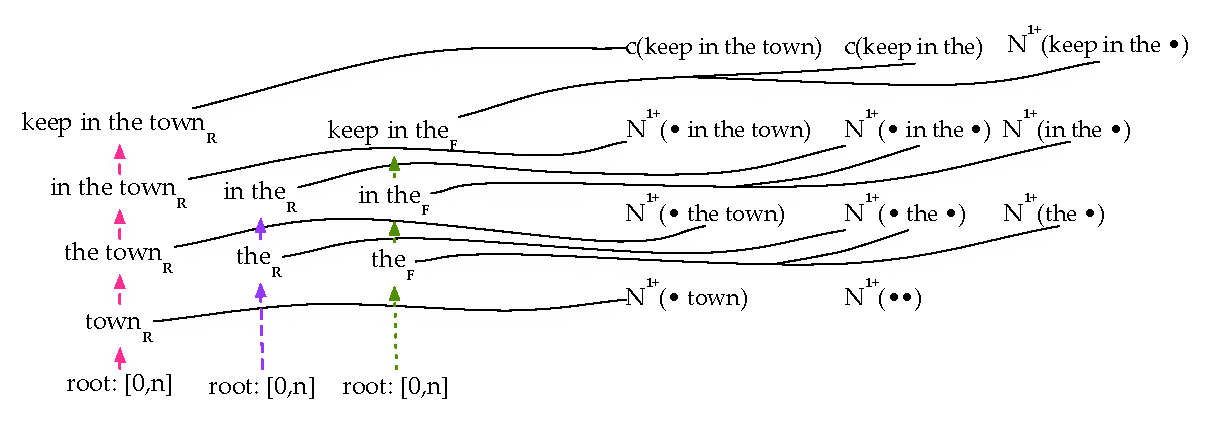
\includegraphics[width=\textwidth]{figures/kn_dual_cst}
\vspace{-3ex}
% \resizebox{1.05\columnwidth}{!}{\hspace{-3ex}
% \begin{tabular}{>{$}c<{$}>{$}c<{$}>{$}c<{$}}
% c(\text{keep in the town})  &  c(\text{keep in the}) &  \nlplus{\text{keep in the} \Bigcdot} \\
% % 1 & 2 & 2 
% %\hline
% \nlplus{\Bigcdot \text{in the town}} & 
% %\quad 1\\
% \nlplus{\Bigcdot \text{in the} \Bigcdot} & 
% %\quad 2 \\
% \nlplus{\text{in the} \Bigcdot} \\
% %& \quad 2 
% \nlplus{\Bigcdot \text{the town}} & 
% %\quad 1\\
% \nlplus{\Bigcdot \text{the} \Bigcdot} & 
% %\quad 4 \\
% \nlplus{\text{the} \Bigcdot} \\
% %& \quad 4  \\ \hline
% \nlplus{\Bigcdot \text{town}} & 
% %\quad 1 \\
% \nlplus{\Bigcdot \Bigcdot} & %\quad 13 \\ % would be 14 but we exclude #$ right?
% \nlplus{\Bigcdot} %& \quad 9  % exclude $ right?
% \end{tabular}}
\caption{Counts required for computing $P(\text{town} | \text{keep in the})$ (right) and the suffix tree nodes required for computing each value (left). The two left-most columns correspond to $\nrfull$ and $\nr$ and are updated using \emph{forward-search} in the reverse \CST, while the righter-most column correspond to $\nf$ and is updated using \emph{backward-search} in the forward \CST. The algorithm is described below in Alg~\ref{alg:pkn}.}
\label{fig-counts-example}
\end{figure*}

\begin{algorithm*}[p]
  \caption{Compute Kneser-Ney probability, $P\big(w_k | w^{k-1}_{k-(n-1)}\big)$
    \label{alg:pkn}}
  \begin{algorithmic}[1]
    \Function{ProbKneserNey}{$\tf, \tr, \ws, n$} 
        \Let{$\nf$}{$\rooot{\tf}$} \Comment{match for context $w^{k-1}_{k-i}$}
        \Let{$\nr$}{$\rooot{\tr}$} \Comment{match for context $w^{k-1}_{k-i}$}
        \Let{$\nrfull$}{$\rooot{\tr}$} \Comment{match for $w^{k}_{k-i}$}
        \Let{$p$}{$1$}
        \For{$i \gets 1 \text{ to } n$}
          \Let{$\nrfull$}{$\forwardsearch{\tr}{\lb{\nrfull}}{\rb{\nrfull}}{w_{k-i+1}}$} \Comment{update matches in \textsc{Cst}s}
          \If{$i > 1$}
             \Let{$\nf$}{$\backwardsearch{\tf}{\lb{\nf}}{\rb{\nf}}{w_{k-i+1}}$} %\Comment{update context match in fwd \CST}
              \If{$i < n$}
             \Let{$\nr$}{$\forwardsearch{\tr}{\lb{\nr}}{\rb{\nr}}{w_{k-i+1}}$} %\Comment{update context match in rev \CST}
          \EndIf
          \EndIf
          \Let{$D$}{lookup discount parameter for $n$-gram}
          \If{$i = n$} % or if s == '<s>' 
                 \Comment{compute the `count' for the full match}
             \Let{$c$}{$\size{\tr}{\nrfull}$} 
             \Let{$d$}{$\size{\tf}{\nf}$}
          \Else
             \Let{$c$}{$\nlplusfunc{\tr}{\nrfull}{\Bigcdot w^{k}_{k-i+1}}$} 
             \Let{$d$}{$\nlplusfrontbackfunc{\tf}{\nf}{\nr}{\Bigcdot w^{k-1}_{k-i+1} \Bigcdot}$} \Comment{precompute $\nlplus{\Bigcdot\Bigcdot}$}
           \EndIf
           \If{$i > 1$}
             \If{$\nf$ is valid} \Comment{compute backoff probability, or backoff for unseen contexts}
                  \Let{$q$}{$\nlplusfunc{\tf}{\nf}{w^{k-1}_{k-i+1} \Bigcdot}$}  \Comment{defined as $0$ for $i=1$}
                  \Let{$p$}{ $\frac{1}{d} \left( \max(c-D, 0)  + D  q  p \right)$} 
               \EndIf
          \ElsIf{$i = 1$}
              \Let{$p$}{$c  / \nlplus{\Bigcdot\Bigcdot}$}
          \EndIf
        \EndFor
      \State \Return{$p$}
    \EndFunction
  \end{algorithmic}
\label{alg-kn-slow}
\end{algorithm*}



\afterpage{\clearpage}

Algorithm~\ref{alg-kn-slow} presents an outline of the approach.
This uses a forward \CST, $\tf$, and a reverse \CST, $\tr$, with three \CST nodes (lines 2--4) tracking the match progress for the full $i$gram ($\nrfull$) and the $i-1$gram context ($\nf, \nr$), $i=1 \ldots n$.
The need to maintain three concurrent searches arises from the calls to size, $\nlplus{\dotpat}$, $\nlplus{\patdot}$ and $\nlplus{\dotpatdot}$ (lines 14,15; 17; 21; and 18, respectively).
Many of these calls impose conditions on the direction of the suffix tree, e.g., such that the edge 
labels and node degree can be used to compute the number of left or right contexts in which a pattern appears. 
The matching process is illustrated in Figure~\ref{fig-counts-example} where the three search nodes are shown on the left, considered bottom to top, and their corresponding count operations are shown to the right.
The $\nlplus{\dotpat}$ calls require a match in the reverse \CST (left-most column, $\nrfull$), while the $\nlplus{\patdot}$ require a match in the forward \CST (right-most column, $\nf$, matching the $(i-1)$gram context). 
The $\nlplus{\dotpatdot}$ computation reuses the forward match while also requiring a match for the $(i-1)$gram context in the reversed \CST, as tracked by the middle column ($\nr$).
Because of the mix of forward and reverse \CSTs, coupled with search patterns that are revealed right-to-left, incremental search in each of the \CSTs needs to be handled differently (lines 7--11).
In the forward \CST, we perform \emph{backward search} to extend the search pattern to the left, which can be computed very efficiently from the BWT in the \CSA \trevor{Complexity?}.
Conversely in the reverse \CST, we must use \emph{forward search} as we are effectively extending the reversed pattern to the right; this operation is considerably more costly \trevor{Complexity? Constraints on type of \CST/\CSA}.

Alg~\ref{alg-kn-slow} uses the  the counts (lines 14 and 17), the denominator (lines 15 and 18) and backoff components (line 21) can be computed.
The probability is initially set in line 24 and updated with each iteration following the KN interpolation in line 22.
Finally, the discount $D$ on line 12 and $\nlplus{\Bigcdot\Bigcdot}$ can be precomputed directly from the \CSTs  thus avoiding several costly computations at runtime. 
The full algorithm is provided in Algorithm~7 in the \supp, which operates by traversing the nodes of the reverse \CST and at each stage computing the number of \ngrams that occur 1--4 times and $\nlplus{\dotpat}$ equal to 1--4, for various lengths of \ngrams (up to a limit, here 10, beyond which we use the values for the largest computed size).
These quantities are used to compute the discount parameters, which are then stored for use in estimation.
Note that this algorithm can be quite slow, although expensive calls to \emph{depth} can be avoided as described before; additionally the calls to \emph{edge} can also be skipped which reduces the runtime by about an order of magnitude, albeit incurring a slight bias to the estimates. \trevor{Complexity?}

\section{Improved single \CST approach}

Just show N1+fb algo; leave rest to supporting material.

\begin{algorithm}
  \caption{Compute two-sided occurrence counts, $\nlplus{\dotpatdot}$, using only forward \CST 
    \label{alg:n1plusfb_wt}}
  \begin{algorithmic}[1]
    \Require{$\nf$ is the node in the forward \CST $\tf$ matching pattern $\alpha$}
    \Require{the \CSA component, $\af$ of $\tf$ is a wavelet tree}
    \Function{N1PlusFrontBack1}{$\tf, \nf, \alpha$} 
        \Let{$o$}{$0$}
        %\If{$\leaf{\tf}{\nf} \, \vee \, \depth{\tf}{\nf} > |\alpha|$}   
        \If{$\depth{\tf}{\nf} > |\alpha|$}   
          \Let{$o$}{$\textsc{N1PlusBack1}{\tr}{\nr}{\dotpat}$}
        \Else
            \For{$\langle l, r, s\rangle \gets \intervalsymbols{\af}{\lb{\nf}}{\rb{\nf}}$}
              \State Some voodoo with Weiner links
               \Let{$o$}{$o +$ something}
            \EndFor
          \EndIf
      \State \Return{$o$}
    \EndFunction
  \end{algorithmic}
\end{algorithm}


%%% Local Variables: 
%%% mode: latex
%%% TeX-master: "cstlm"
%%% End: 
